\section{Fazit und Ausblick}
\subsection{Fazit}
\subsubsection{Fazit Rundfahrt}
\subsubsection{Fazit Schildererkennung}
\subsection{Ausblick}
\subsubsection{Ausblick Rundfahrt}
\subsubsection{Ausblick Schildererkennung}
Momentan erkennt das neuronale Netz vier Schilder, doch das Roboterauto reagiert noch nicht auf diese und erkennt sie nur. Das Team hat bereits einen Zustandsautomaten, siehe Abbildung \ref{fig:zustandsautomat} f\"ur die Weiterverarbeitung der Schildererkennung entwickelt und in C++ realisiert.
\begin{figure}[h]
	\centering
	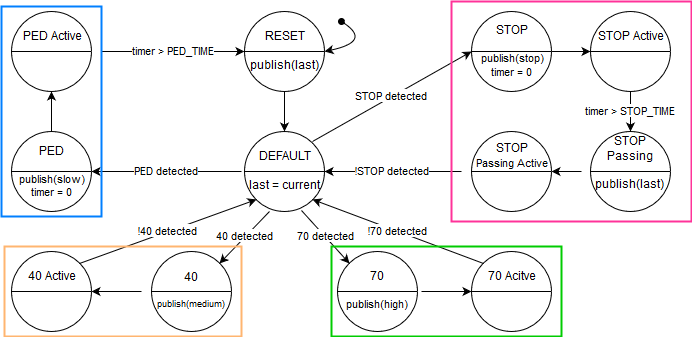
\includegraphics[width = 1\textwidth]{images/StateMachine.png}
	\caption{Zustandsautomat f\"ur die Schildererkennung}
	\label{fig:zustandsautomat}
\end{figure}
\\
Wenn das neuronale Netz ein Schild oder mehrere Schilder erkennt, dann werden diese \"uber ein ROS-Topic ver\"offentlicht. Diese erkannten Schilder werden zun\"achst darauf \"uberpr\"uft, welches das n\"achste Schild im Abstand zum Roboterauto ist und ob der Abstand zu dem Schild klein genug ist, um darauf reagieren zu m\"ussen. Falls dies der Fall ist, so wird das entsprechend n\"achste Schild als Ereignis an den Zustandsautomaten weitergegeben, falls nicht wird das Ereignis weitergegeben, dass kein Schild erkannt wurde.
\\\\Die Bedeutungen der einzelnen K\"urzel des Zustandsautomaten werden folglich erkl\"art:
\begin{itemize}
\item Geschwindigkeitenereignisse werden mit den Konstanten \textbf{\textit{stop}}, \textbf{\textit{slow}}, \textbf{\textit{medium}} und \textbf{\textit{high}} beschrieben, wobei gilt:
\begin{align}
\begin{split}
\label{vel_vergleich}
0 = stop < slow < medium < high
\end{split}
\end{align}

\item \textbf{\textit{current}} und \textbf{\textit{last}} sind Variablen und beschreiben welches Geschwindigkeitsereignis gerade in diesem Moment und welches Geschwindigkeitsereignis zuvor galt. Beide haben den Initialwert \textbf{\textit{medium}}.

\item Die Funktion \textbf{\textit{publish(x)}} ver\"offentlicht ein Geschwindigkeitsereignis \"uber ein ROS-Topic, welches dann von anderen ROS-Nodes abonniert werden kann.

\item Die Zeitkonstanten \textbf{\textit{PED\underline{\ }TIME}} und \textbf{\textit{STOP\underline{\ }TIME}} stellen einen Zeitwert in Sekunden dar.

\item \textbf{\textit{timer}} ist ein Z\"ahler und z\"ahlt die Sekunden hoch.

\item \textbf{\textit{STOP}}, \textbf{\textit{PED}}, \textbf{\textit{40}} und \textbf{\textit{70}} sind Schildereignisse, welche der Zustandsautomat als Eingabe empf\"angt. 

\item Die Transitionsbedingung \textbf{\textit{x detected}} schaltet dann, wenn das entsprechende Schildereignis von dem Zustandsautomaten als Eingabe empfangen wurde.

\item Der Zustand \textbf{\textit{RESET}} stellt den Initialzustand dar und ver\"offentlicht das Geschwindigkeitsereignis \textbf{\textit{last}}.

\item Der Zustand \textbf{\textit{DEFAULT}} ist ein Zustand, welcher in jedem Ereigniszyklus einmal ausgel\"ost wird und das Geschwindigkeitsereignis \textbf{\textit{current}} auf \textbf{\textit{last}} setzt.

\end{itemize}


\begin{figure}[h]
\begin{minipage}[t]{4cm}
\vspace{0pt}
\centering
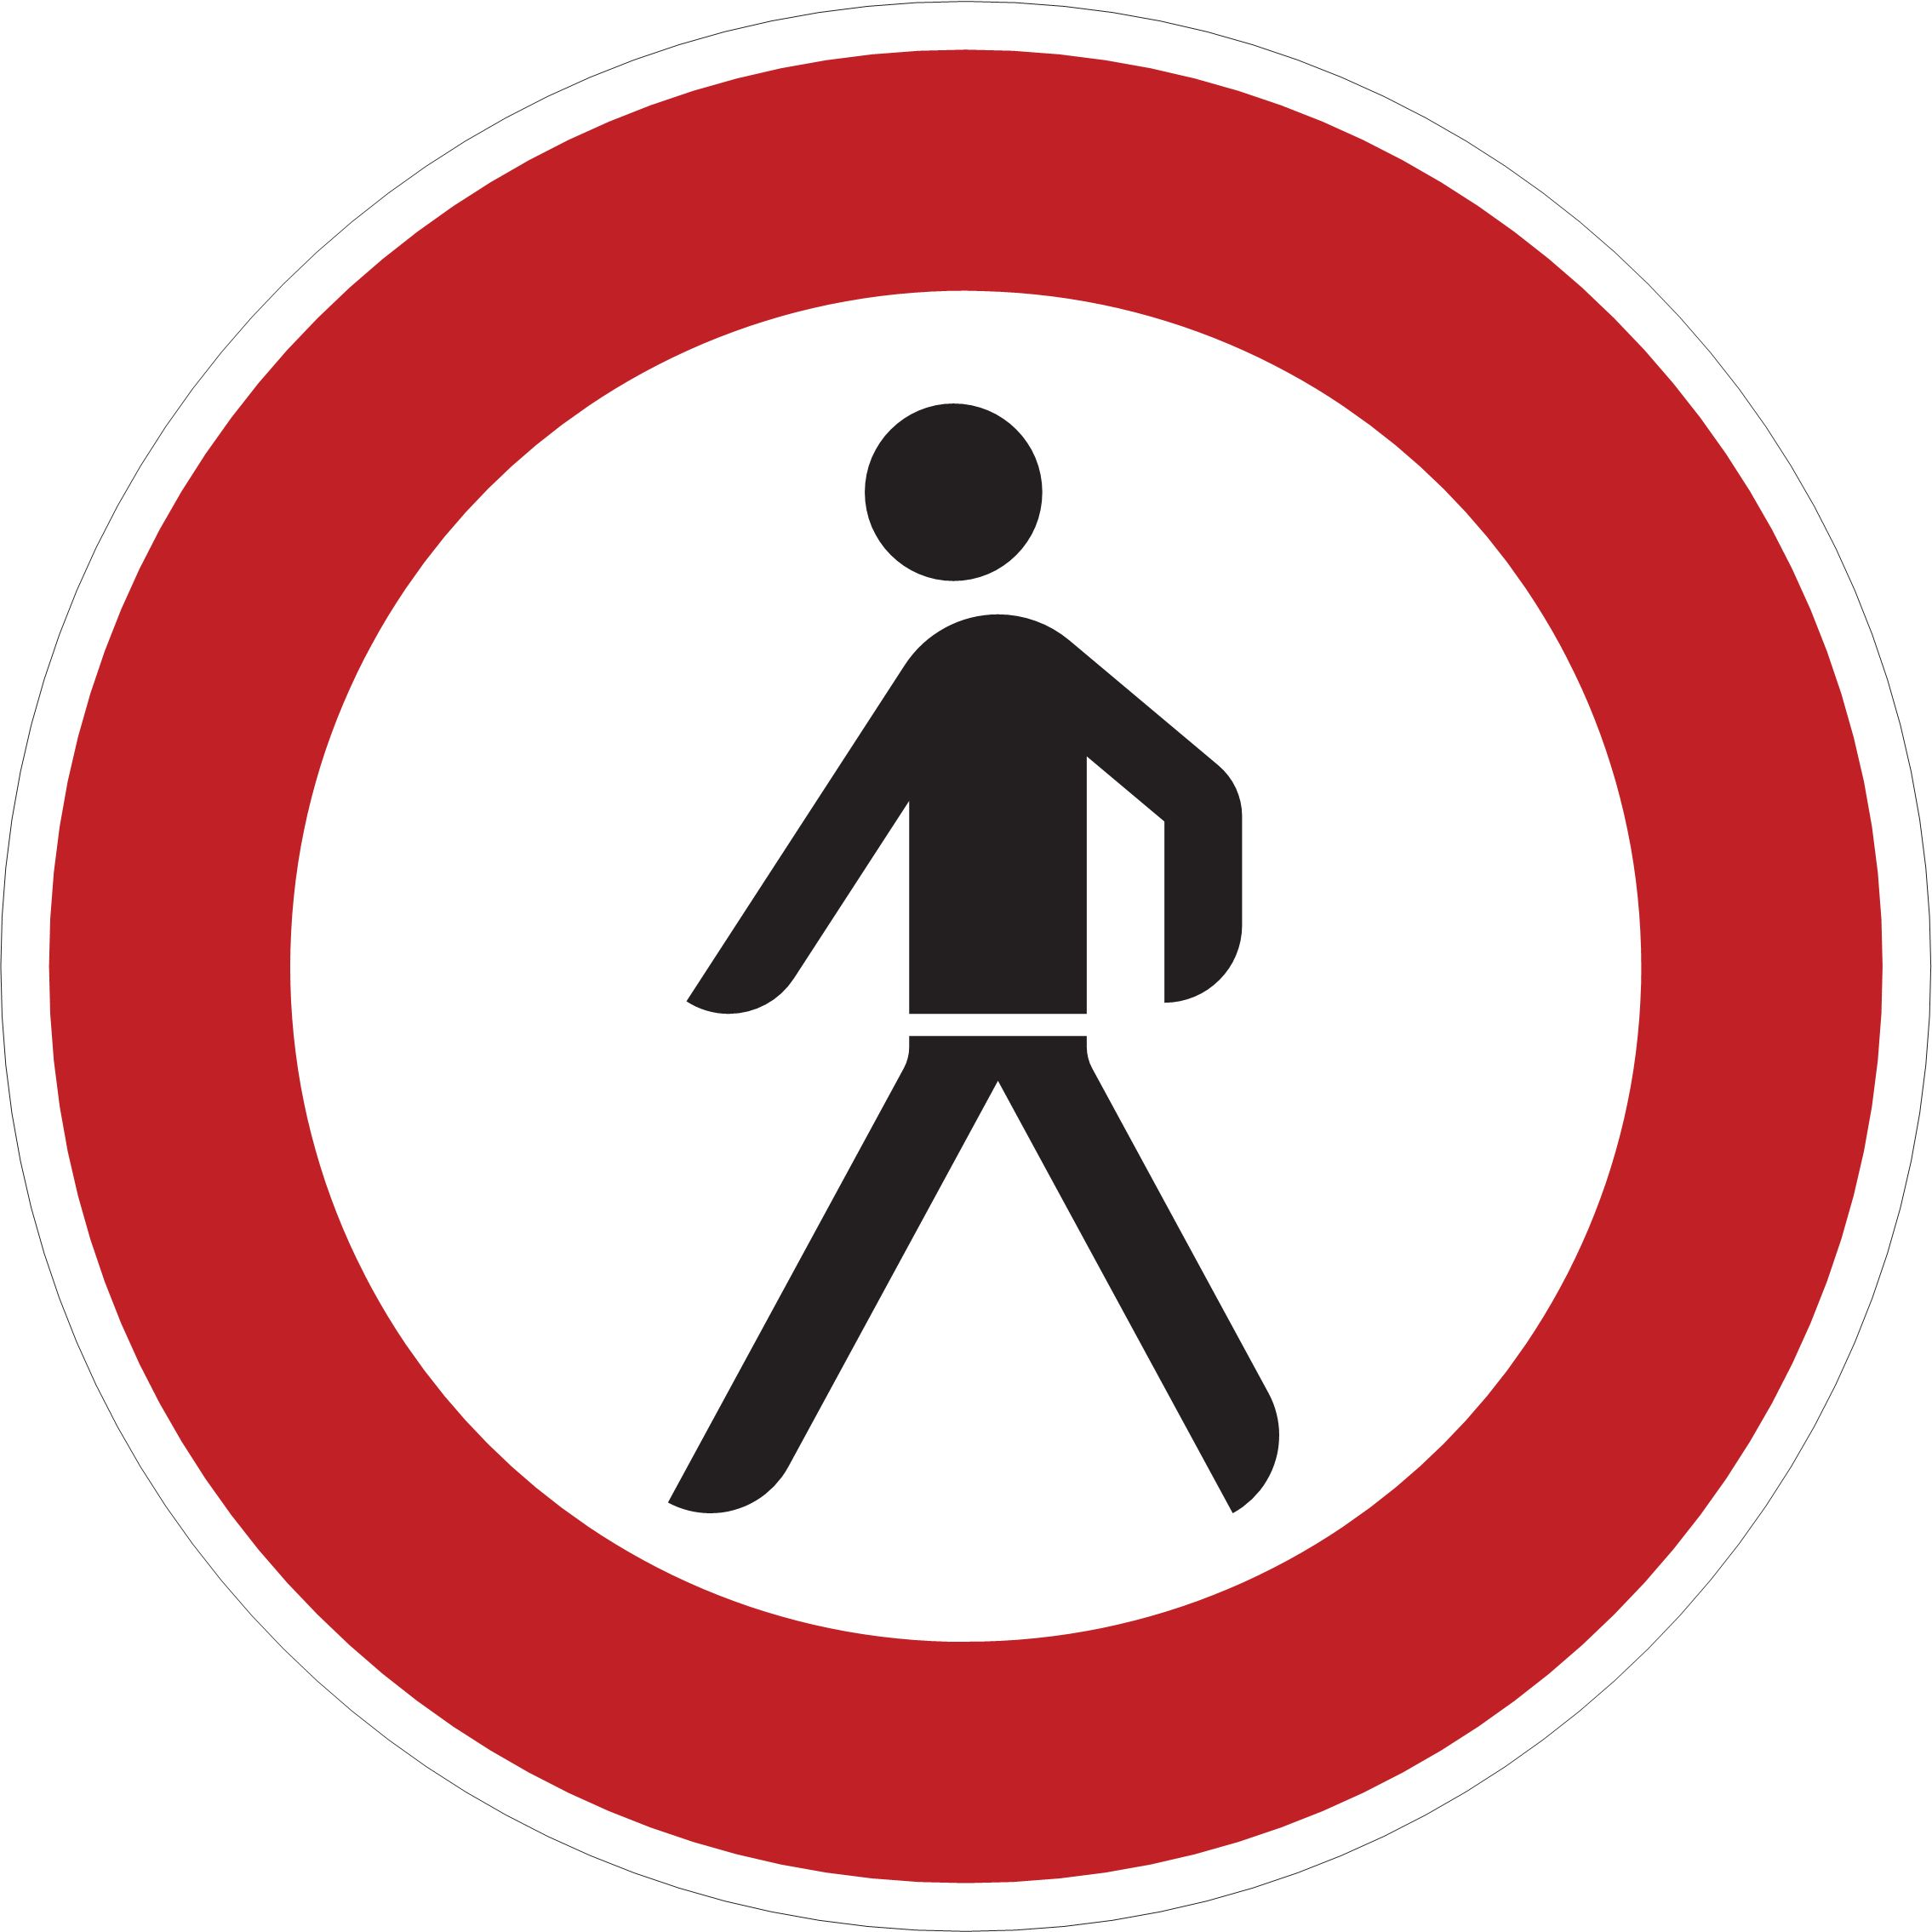
\includegraphics[scale=0.07]{images/PED.jpg}
\caption{Verbot f\"ur Fu\ss{}g\"anger}
\label{fig:PED}
\end{minipage}
\hfill
\begin{minipage}[t]{10cm}
\vspace{0pt}
\begin{itemize}
\item Der blau markierte Bereich im Zustandsautomaten beschreibt, was das Schild "Verbot f\"ur Fu\ss{}g\"anger"\ bewirkt. Das Schild wird als "Vorsicht Fu\ss{}g\"anger"\  interpretiert.

\item Wenn als Eingabe \textbf{\textit{PED}} empfangen wird, wird ein Z\"ahler gestartet und das Geschwindigkeitsereignis \textbf{\textit{slow}} ver\"offentlicht.

\item Sobald der Z\"ahler \textbf{\textit{PED\underline{\ }TIME}} \"uberschritten wird, wird das Geschwindigkeitsereignis auf \textbf{\textit{last}} zur\"uckgesetzt und zur\"uck auf den Status \textbf{\textit{DEFAULT}} geschaltet.
\end{itemize}
\end{minipage}
\end{figure}


\begin{figure}[h]
\begin{minipage}[t]{4cm}
\vspace{0pt}
\centering

\includegraphics[scale=0.04]{images/STOP.jpg}
\caption{Stoppschild}
\label{fig:PED}
\end{minipage}
\hfill
\begin{minipage}[t]{10cm}
\vspace{0pt}
\begin{itemize}
\item Der magenta markierte Bereich im Zustandsautomaten beschreibt, was das Schild "Stoppschild"\ bewirkt.

\item Wenn als Eingabe \textbf{\textit{STOP}} empfangen wird, wird ein Z\"ahler gestartet und das Geschwindigkeitsereignis \textbf{\textit{stop}} ver\"offentlicht.

\item Sobald der Z\"ahler \textbf{\textit{STOP\underline{\ }TIME}} \"uberschritten wird, wird das Geschwindigkeitsereignis auf \textbf{\textit{last}} zur\"uckgesetzt. Hierbei wird darauf geachtet, dass der Zustandsautomat erst dann auf \textbf{\textit{DEFAULT}} weiterschaltet, wenn ein Ereignis au\ss{}er \textbf{\textit{STOP}} empfangen wird, um unendliche Schleifen zu vermeiden.
\end{itemize}
\end{minipage}
\end{figure}


\begin{figure}[h]
\begin{minipage}[t]{4cm}
\vspace{0pt}
\centering

\includegraphics[scale=0.07]{images/40.png}
\caption{Zul\"assige H\"ochstgeschw.}
\label{fig:PED}
\end{minipage}
\hfill
\begin{minipage}[t]{10cm}
\vspace{0pt}
\begin{itemize}
\item Der orange markierte Bereich im Zustandsautomaten beschreibt, was das Schild "Zul\"assige H\"ochstgeschwindigkeit 40km/h"\ bewirkt.

\item Wenn als Eingabe \textbf{\textit{40}} empfangen wird, wird das Geschwindigkeitsereignis \textbf{\textit{medium}} ver\"offentlicht.

\item Sobald ein Geschwindigkeitsereignis au\ss{}er \textbf{\textit{40}} empfangen wird schaltet der Zustandsautomat zur\"uck auf den Status \textbf{\textit{DEFAULT}}
\end{itemize}
\end{minipage}
\end{figure}


\begin{figure}[h]
\begin{minipage}[t]{4cm}
\vspace{0pt}
\centering

\includegraphics[scale=0.06]{images/70.png}
\caption{Zul\"assige H\"ochstgeschw.}
\label{fig:PED}
\end{minipage}
\hfill
\begin{minipage}[t]{10cm}
\vspace{0pt}
\begin{itemize}
\item Der gr\"un markierte Bereich im Zustandsautomaten beschreibt, was das Schild "Zul\"assige H\"ochstgeschwindigkeit 70km/h"\ bewirkt.

\item Wenn als Eingabe \textbf{\textit{70}} empfangen wird, wird das Geschwindigkeitsereignis \textbf{\textit{high}} ver\"offentlicht.

\item Sobald ein Geschwindigkeitsereignis au\ss{}er \textbf{\textit{70}} empfangen wird schaltet der Zustandsautomat zur\"uck auf den Status \textbf{\textit{DEFAULT}}
\end{itemize}
\end{minipage}
\end{figure}
